% !TEX root = trackjet_intnote.tex

This section gives an overview of the sources of systematic uncertainties on the \pp\ and \pbpb\ charged particle spectra associated with jet. The sources of systematic uncertainties in the measurement are the following and are further described below:

\begin{itemize}

\item Jet energy scale

\item Jet energy resolution

\item Track selection

\item Truth track definition

\item Detector material description in simulation

\item Tracking in dense environments

\item Fake track subtraction

\item Track momentum

\item Unfolding

\item Underlying event contribution

%\item MC non-closure

\end{itemize}


The systematic uncertainties on the \Rdptr\ distributions for a selection of track \pt\ ranges (1.0--1.6 \GeV, 2.5--4.0 \GeV, 6.3--10 \GeV) in jets with \pt\ in the 126--158 \GeV\ range are shown in Figure~\ref{fig:rdptr_sys_uncert}. All uncertainties are assumed to be uncorrelated, and thus are combined in quadrature to give the total systematic uncertainty. The systematic uncertainties for other jet \pT\ interval as show in appendix\ref{sec:appendixA}. 

\begin{figure}
\centering{
\begin{tabular}{cc}
	 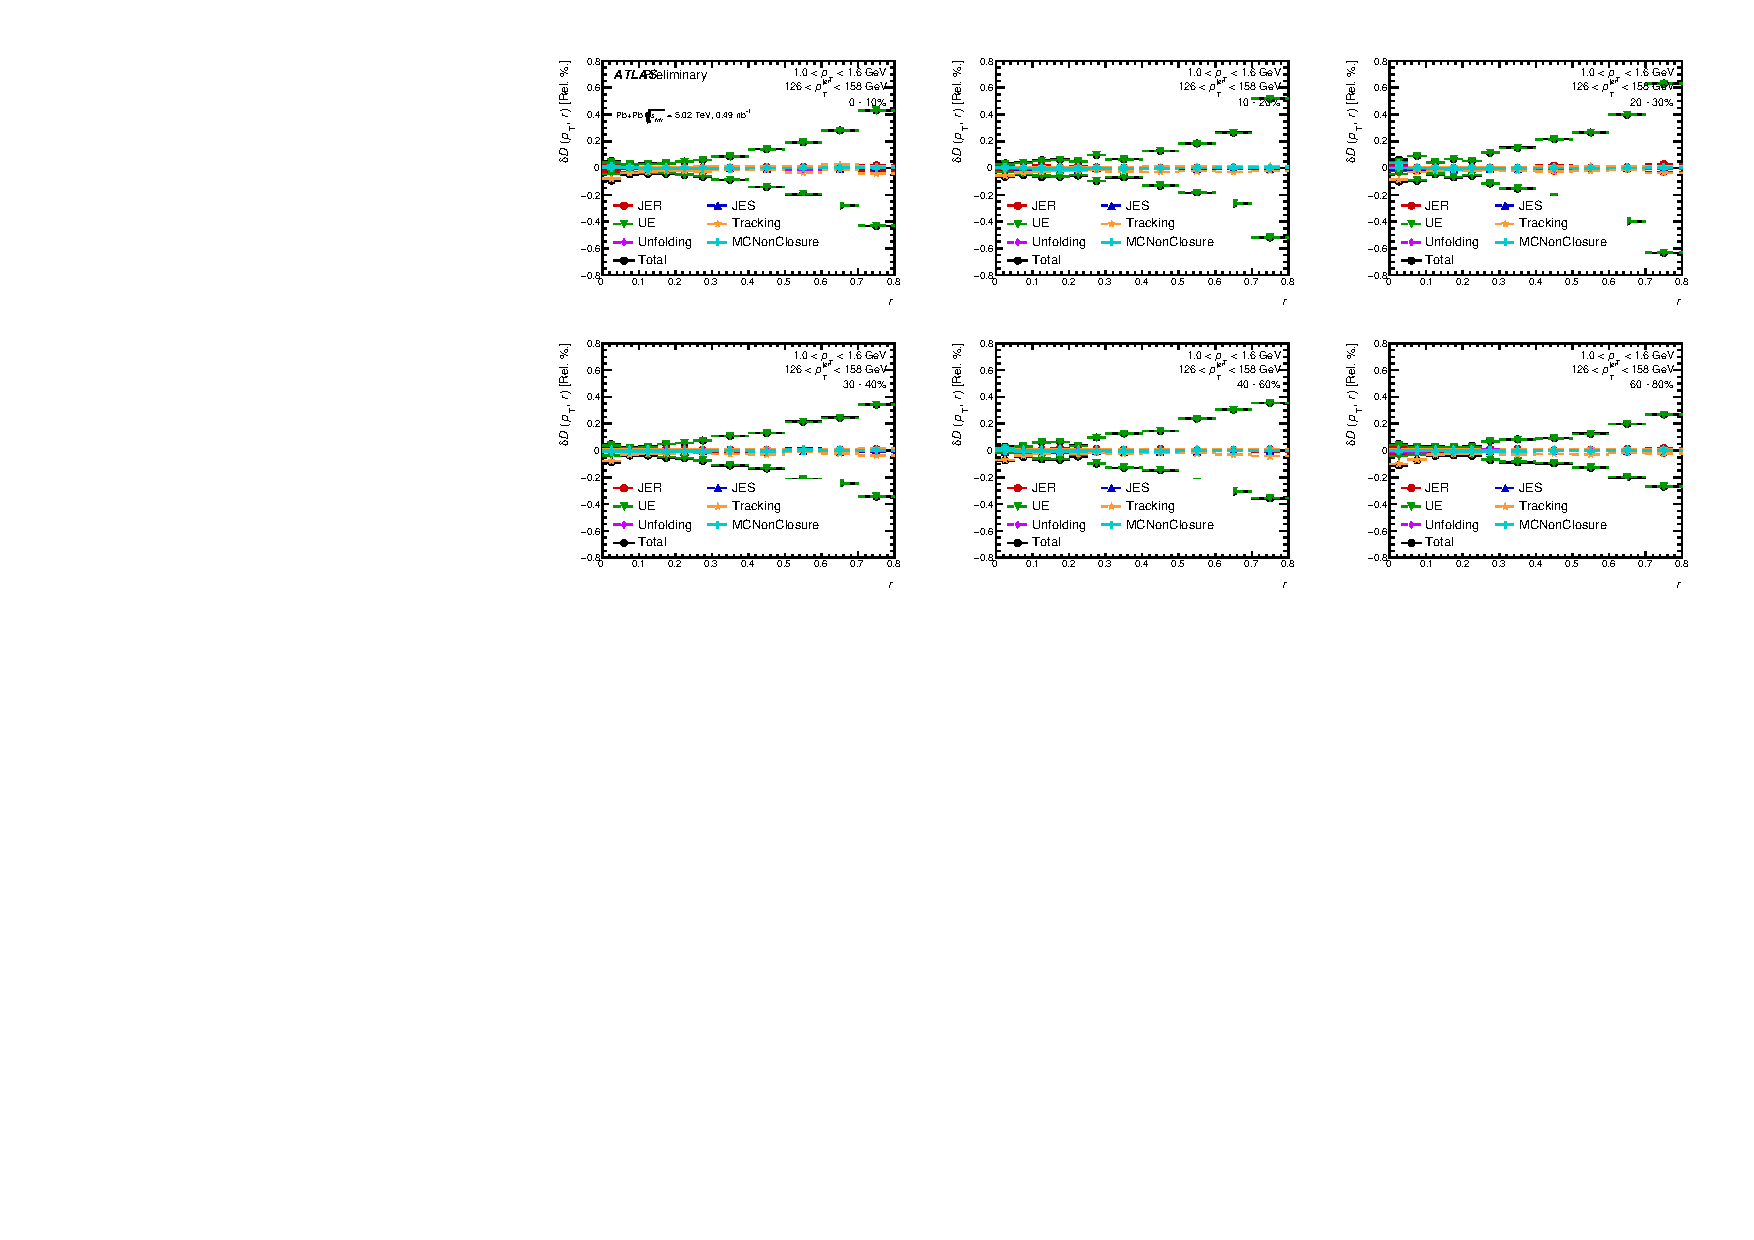
\includegraphics[page=1, width=0.85\textwidth]{figures_systematics/ChPS_dR_sys_PbPb_error} \\
	 \includegraphics[page=3, width=0.85\textwidth]{figures_systematics/ChPS_dR_sys_PbPb_error} \\
	 \includegraphics[page=5, width=0.85\textwidth]{figures_systematics/ChPS_dR_sys_PbPb_error} \\
\end{tabular} }
   \caption{A summary of the systematic uncertainties on \RDptr\ distributions for different track \pt, bins, for jets with \pt\ 125--158 \GeV\ , as a function of \rvar\ for different centrality bins. The uncertainties from the JES, JER, UE, and Tracking  are shown, along with the total systematic uncertainty from all sources. }
      \label{fig:rdptr_sys_uncert}
\end{figure}




The systematic uncertainties have been evaluated separately for \Dptr\ distributions and for their ratios, as a function of jet \pT\ for \pp\ and \pbpb\ collisions. 
For each systematic variation, the entire unfolding procedure is repeated (2D unfolding of the fragmentation
functions as a function of \ptjet\, the 1D unfolding of the single \ptjet\ spectrum and the bin-by-bin correction for position resolution). This is necessary because the jets are in both the 2D and the 1D unfolding procedures and must be treated in a consistent manner throughout the analysis (e.g. a shift in the JES should 
shift jets in the fragmentation functions as a function of \ptjet\ in the same manner
that the single jet spectrum itself is shifted).
The positive relative uncertainty was used to calculate the upper bound of the systematic uncertainty, whereas the negative relative uncertainty was used to calculate the lower bound. All sources of systematic uncertainty discussed in this section are treated as mutually uncorrelated and are combined in quadrature to obtain the total systematic uncertainty. 

\subsection{Jet energy scale uncertainty}

The uncertainty on the JES for heavy ion jets has two parts.  The first part is taken from
the \pp\ JES uncertainties for EMTopo jets and the second part is specific to the heavy ion jets
and collision energies (for flavor related uncertainties).  For the \pp\ part we use the globally reduced
set of 19 nuisance parameters described in Ref.~\cite{JESuncertaintytwiki}. Nuisance parameters that are not applicable for HI jet collections (pileup, b-jets, flavor and MC non closure) are removed or replaced (flavor uncertainties). The heavy ion specific components are from the cross calibration~\cite{cc2015} and the jet
flavor uncertainties at 5.02~TeV~\cite{pPbIntNote}.  For each component of the variation
the response matrices are regenerated with the shifted \ptjet:
\begin{equation}
   \pT^{\star,\mathrm{reco}} = \pT^{\mathrm{reco}} (1\pm U^{\mathrm{JES}}(\pT , \eta)).
\end{equation}
The data is then re-unfolded with these response matrices and the variation in the fragmentation 
functions is taken as the systematic uncertainty.

 The centrality dependent uncertainty on the JES was evaluated by shifting the jet \pt\ of all measured jets up and down by shift between 0\% and 0.5\%. The magnitude of the shift depends on the centrality in the way that the uncertainty on the jet \pt\ is 0.5\% in 1\% most central collisions and than linearly decreases to 0\% in 60\% peripheral bin. The size of the shift reflects the uncertainty on the JES evaluated as using the $r-$track study where the sum of \pT\ of the tracks associated to a reconstructed jet is compared to the reconstructed jet \pT\ in ratio that is than compared between PbPb data and MC~\cite{HIjesnote,PbPbRaaNote}.

\subsection{Jet energy resolution}
To account for systematic uncertainties due to disagreement between the jet energy resolution in data and MC, the unfolding procedure was repeated with a modified response matrix. The matrix was generated by repeating the MC study with modifications to the $\Delta \pt$ for each matched truth-reconstructed jet pair. 



     The procedure to generate modified migration matrices follows the standard procedure applied in p+p jet measurements 
     and is used for both the \pp\ and \pbpb\ collisions. 
     The $\texttt{JetEnergyResolutionProvider}$ tool~\cite{JERUncertaintyProviderRun2} was used to 
     retrieve uncertainty on the fractional resolution, $\sigma^{\mathrm{syst}}_{\mathrm{JER}}$ as a function of jet $\pt$ and $\eta$. An additional HI jet specific uncertainty was derived~\cite{cc2015} (this
     uncertainty is for the HI jet collections and thus is applied to the jets in both \pp\ and \pbpb\
     collisions). 
     The full JER uncertainty on 2015 \pp\ data is shown also in Ref.~\cite{Aad:1696485}

     The jet $\pt^{\mathrm{reco}}$ was then smeared by
     \begin{equation}
	\pt^{\star, \mathrm{reco}} = \pt^{\mathrm{reco}}\times \mathcal{N}(1,\sigma^{\mathrm{eff}}_{\mathrm{JER}})\,,
     \end{equation}
     where $\mathcal{N}(1,\sigma^{\mathrm{eff}}_{\mathrm{JER}})$ is the normal distribution with the effective resolution $\sigma^{\mathrm{eff}}_{\mathrm{JER}}=\sqrt{(\sigma_{\mathrm{JER}} + \sigma^{\mathrm{syst}}_{\mathrm{JER}})^{2} - \sigma_{\mathrm{JER}}^{2}}$. As this smearing is random the procedure is repeated 10 times.

     %The systematic uncertainties on the \Dptr\ distributions decreases with decreasing \pt\ and increasing jet \pT. The typical systematic uncertainty originating from JER changes varies from 10\% to 1\% depending on the jet \ET\ and $z$. 


\subsection{Track selection and efficiency}

\paragraph{Track selection}  This uncertainty was estimated by tightening the tracking cuts by adding the cuts
on the significance of $d_0$ and $z_0$ as described in the Section~\ref{sec:trackselection}.  
The entire analysis is redone with these track selections and the difference from the nominal analysis is taken as the systematic uncertainty. 


%\paragraph{Tracking efficiency fits}  This uncertainty comes from the statistical uncertainty on the fits
%used to parameterize the efficiency corrections.  Since this uncertainty is largely from the statistical 
%fluctuations of the uncertainty points it is taken to be uncorrelated between \pp\ and \pbpb. 
%This uncertainty is not yet added to the total systematics for fragmentation functions in \pbpb\ collisions.

\paragraph{Truth track definition}  
This uncertainty quantifies robustness of the matching of reconstructed to truth particles.
The uncertainty is taken as a difference in the final results obtained with  $MCprob>$ 0.3 
and results obtained with $MCprob>$ 0.5. 


\paragraph{Detector material description in simulation}
The uncertainty on the inner detector material
varies with \pttrk\ and \etatrk\ from 0.5\% to 2.0\%~\cite{ref:tracktwiki} on the efficiency correction.  


\paragraph{Tracking in dense environments}
There is a 0.4\% uncertainty on the efficiency due to tracking in dense environments (the core of the jet)~\cite{ref:tracktwiki}.


\paragraph{Fake rate}
The uncertainty on the rate of fake tracks is 30\% independent of \pttrk\ and \etatrk~\cite{ref:tracktwiki}. 

\paragraph{Uncertainty on the track momentum}
To account for a possible miss-alignment in \pp\ and \PbPb\ data, the reconstructed \pT\ of each track (corrected first as described in section~\ref{Sec:Trackmomentumcorrection}) was changed according to~\cite{TrackingRec}:

\begin{equation}
\pt \rightarrow \pt \times (1 + q \times \pt \delta_{sagitta}(\eta, \phi))^{-1},
\end{equation}
where $q$ is charge of the track and $\delta_{sagitta}(\eta, \phi)$ is uncertainty on the track curvature. The uncertainty derived for 5.02~TeV \pp\ and \PbPb\ data is included in InDetTrackSystematicsTools-00-00-19. Due to statistical origin of the uncertainty the resulting systematic uncertainty is symmetrized. 

%The resulting systematic uncertainty is $<<1$\% for low and intermediate $z$ and \pT\ and reaches up to 4\% at high $z$. As the source of the shift is present both in \pp\ and \PbPb\ it does partially cancel in the ratios.  

\subsection{Systematic uncertainty due to unfolding}
The systematic uncertainty associated with the unfolding is connected with the sensitivity of the unfolding procedure to the choice of the input distributions. The systematic is evaluated by generating response matrices from the MC distributions with an additional reweighting factor so as to match the jet and charged particle distributions in data, and then unfolding the data using these modified response matrices. The reweighting of the track \pt\ has a minimal effect because of the good track momentum resolution in the kinematic region of interest. The uncertainty is evaluated by comparing the nominal result with the reweighted result, and is considered to be uncorrelated between \pbpb\ and \pp.


\subsection{Systematic uncertainty due to the UE event subtraction}
The systematic uncertainty associated with the estimation of the UE is estimated by comparing the UE evaluated by two different methods. The UE estimated using the MB events that are described in the section~\ref{sec:cuts_corrections} is compared to UE estimated using using random cone method that was used in the in the previous study on inclusive jet fragmentation functions. A short summary of the method follows. More details can be found in Ref.~\cite{PbPb5TeVIntNote}. 

The UE contribution is determined using a grid of \RFour\ cones spanning the full coverage of the inner detector. The method is applied on events containing jets included in the analysis. The cones have a fixed distance between their centers chosen such that the inner detector acceptance is uniformly covered while avoiding overlaps. Any cone having a charged particle with $\pT>10$~\GeV\ or overlapping with a reconstructed jet with $\ptjet > 90$ \GeV\  is assumed to be associated with a 
hard process and is excluded from the UE estimation.

The resulting UE charged-particle yields,  $\fd \nchUE/ \fd \z$ or $\fd \nchUE/ \fd \pttrk$, are evaluated over $1 < \pttrk < 10$~\GeV\ according to:
	\begin{eqnarray}
	\label{eq:background1}
	\dfrac{\fd \nchUE}{ \fd \pttrk} &=&
	\dfrac{1}{\Ncone}
        \dfrac{1}{\varepsilon(\pttrk,\etatrk)}
        \dfrac{\Delta N_{\mathrm{ch}}^{\mathrm{cone}}(\pttrk,\ptjet,
	  \yjet)}{\Delta \pttrk}.
	\end{eqnarray}
The \Ncone\ is the number of background cones used in the UE determination of a given jet, $\Delta N_{\mathrm{ch}}^{\mathrm{cone}}$ represents the number of charged particles summed over all background cones, and $\Delta R$ represents the distance between the center of a cone and the direction of a given charged particle. The $\varepsilon(\pttrk,\etatrk)$ is the efficiency for reconstructing charged particles estimated as a function of \pttrk\ and \etatrk\ without requirement on the track-to-jet association.

\begin{figure}
\centering{
\begin{tabular}{cc}
	 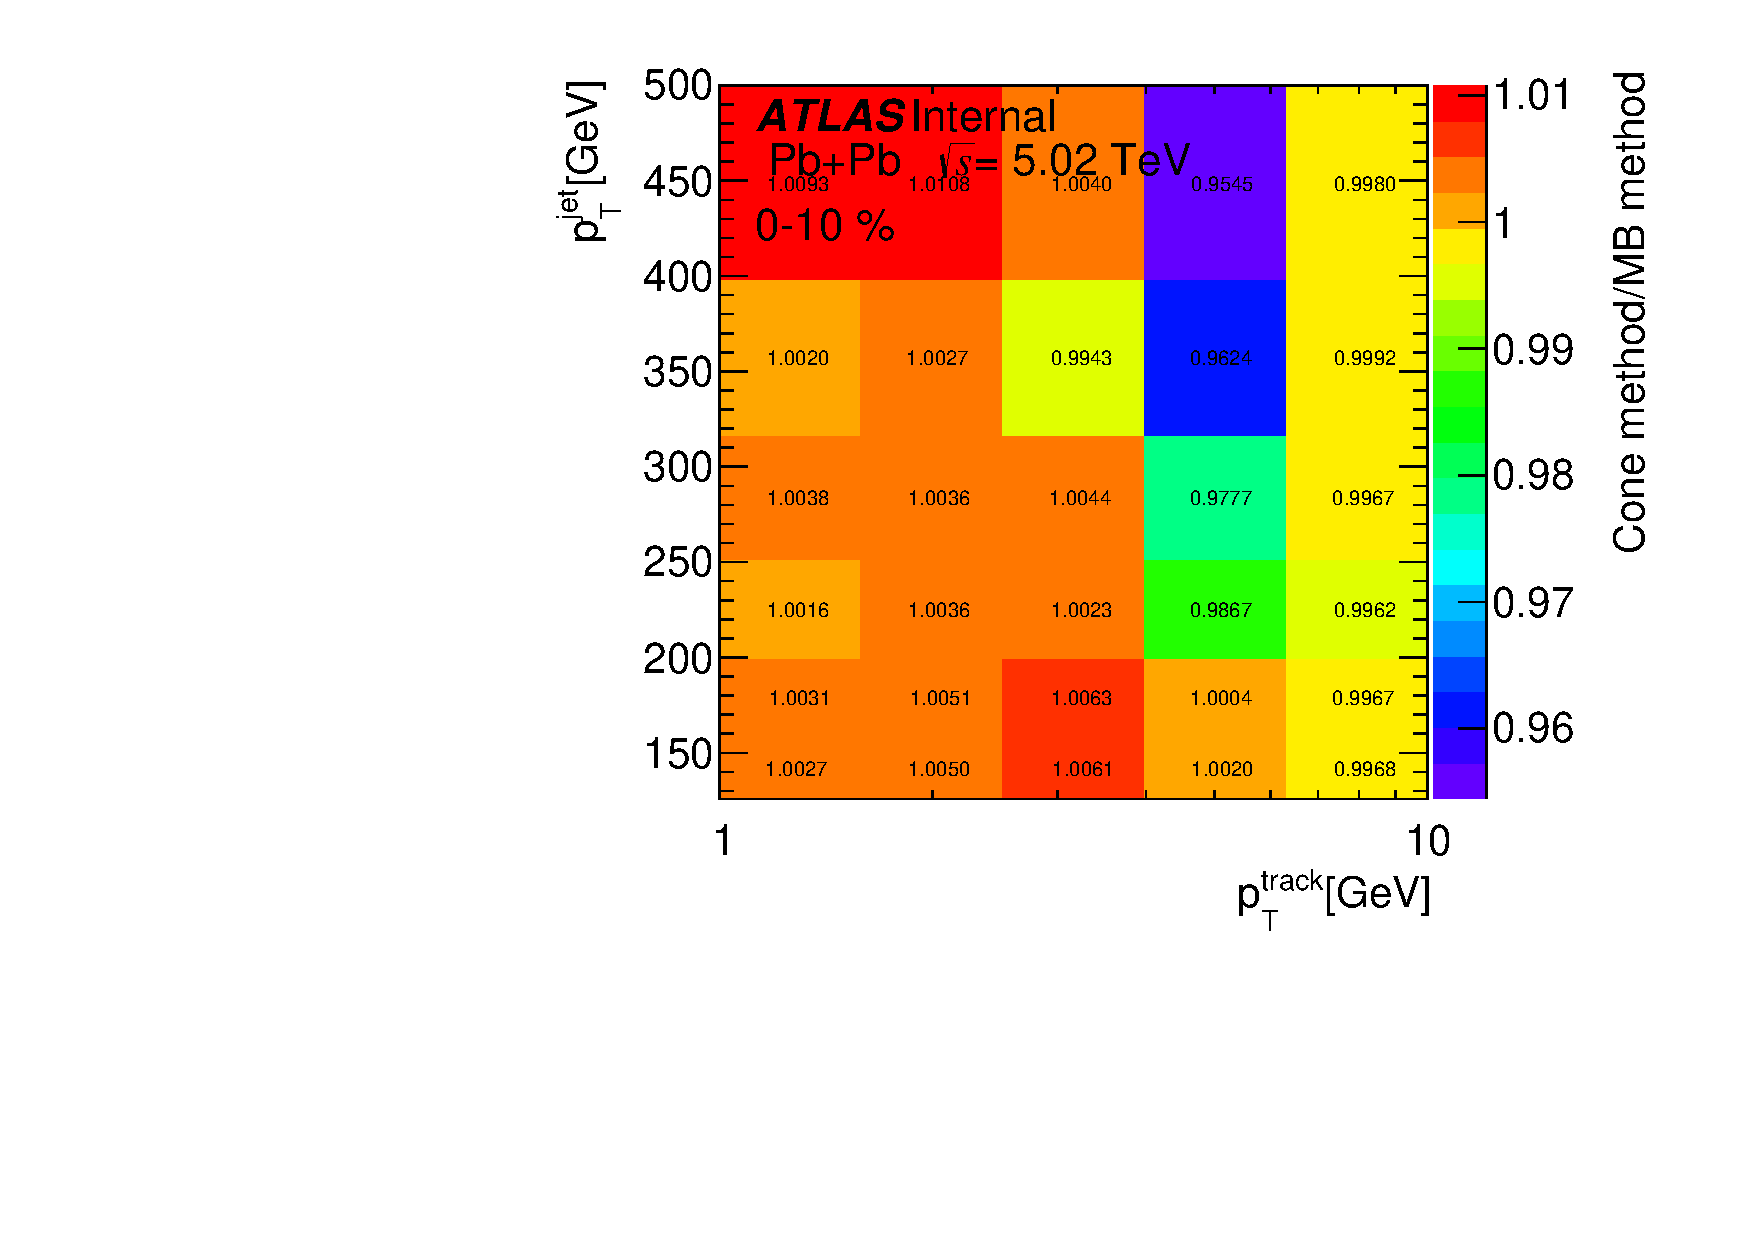
\includegraphics[width=0.55\textwidth]{figures_systematics/h_UE_comparison_cent0} &
	 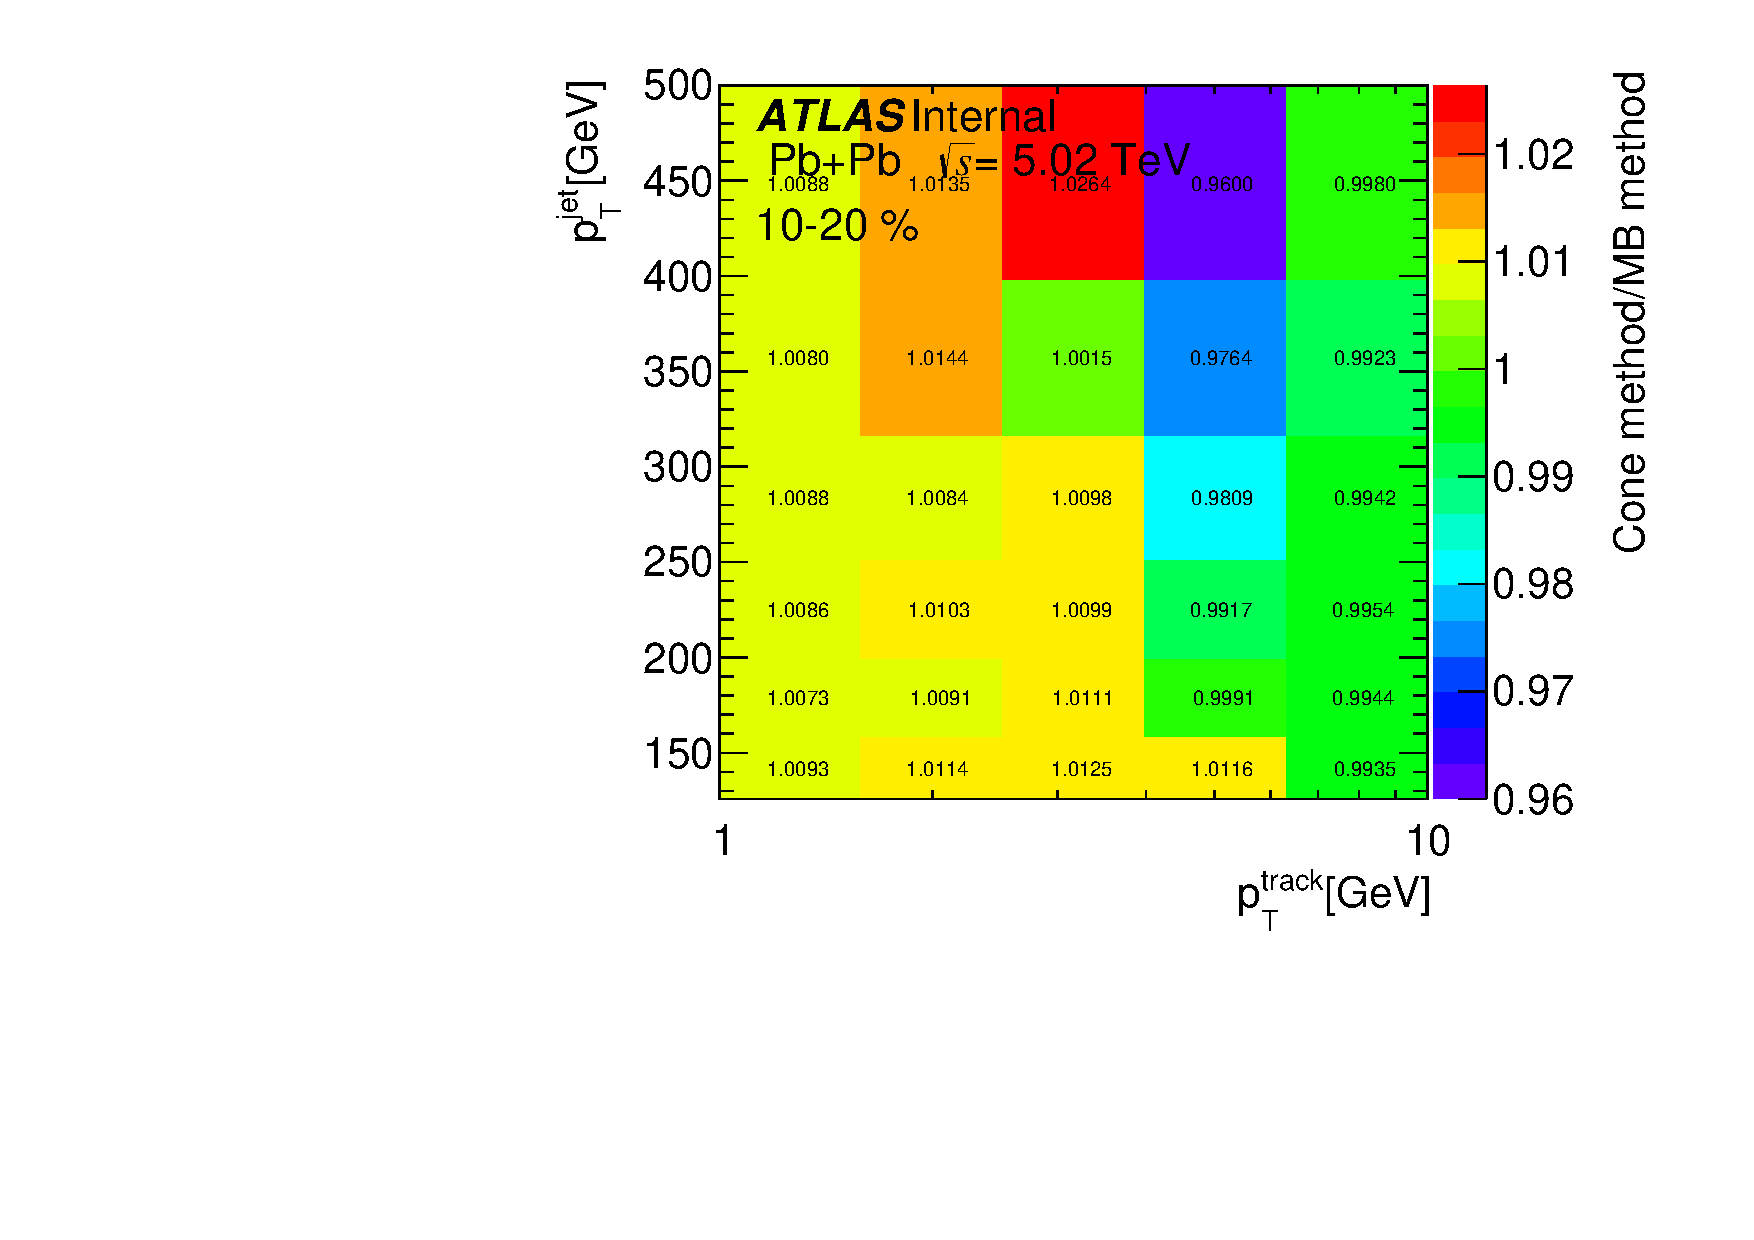
\includegraphics[width=0.55\textwidth]{figures_systematics/h_UE_comparison_cent1} \\
	 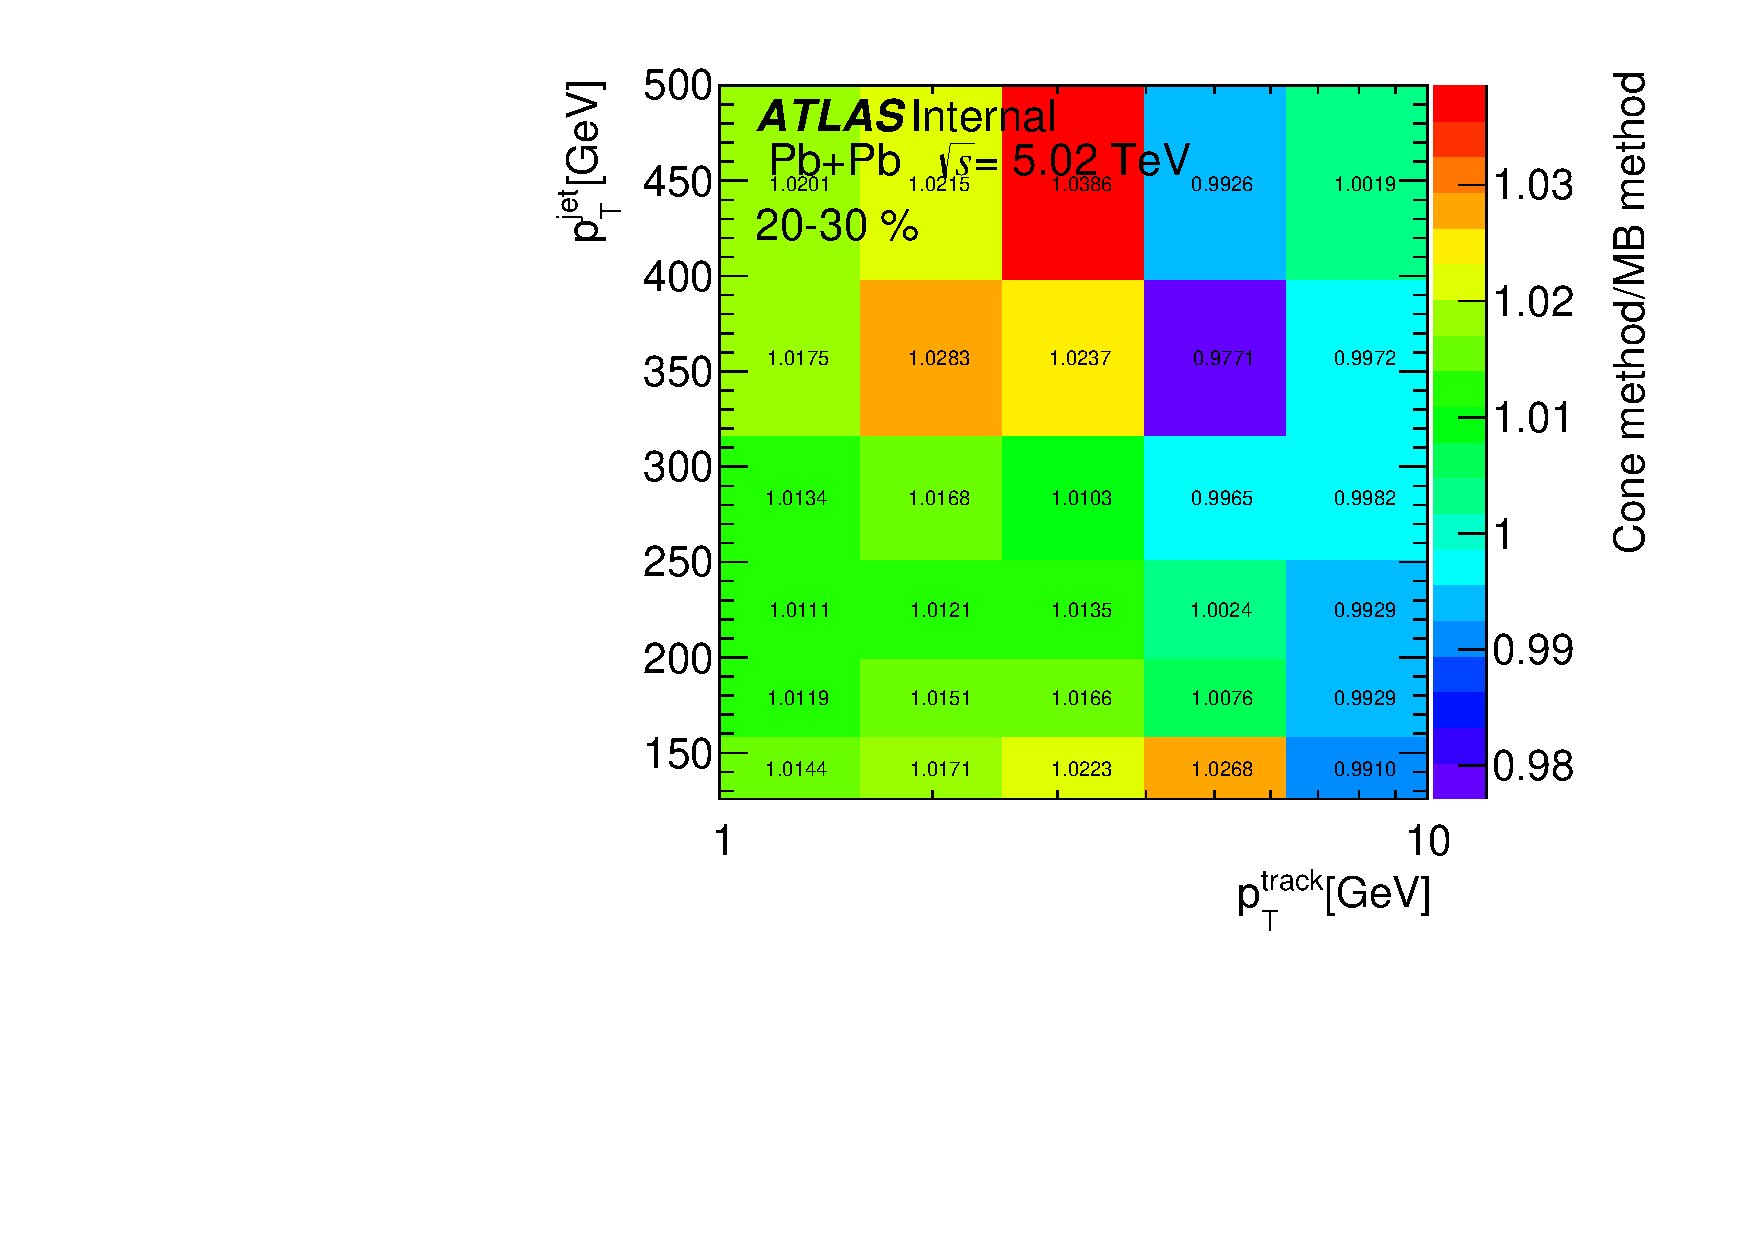
\includegraphics[width=0.55\textwidth]{figures_systematics/h_UE_comparison_cent2} &
	 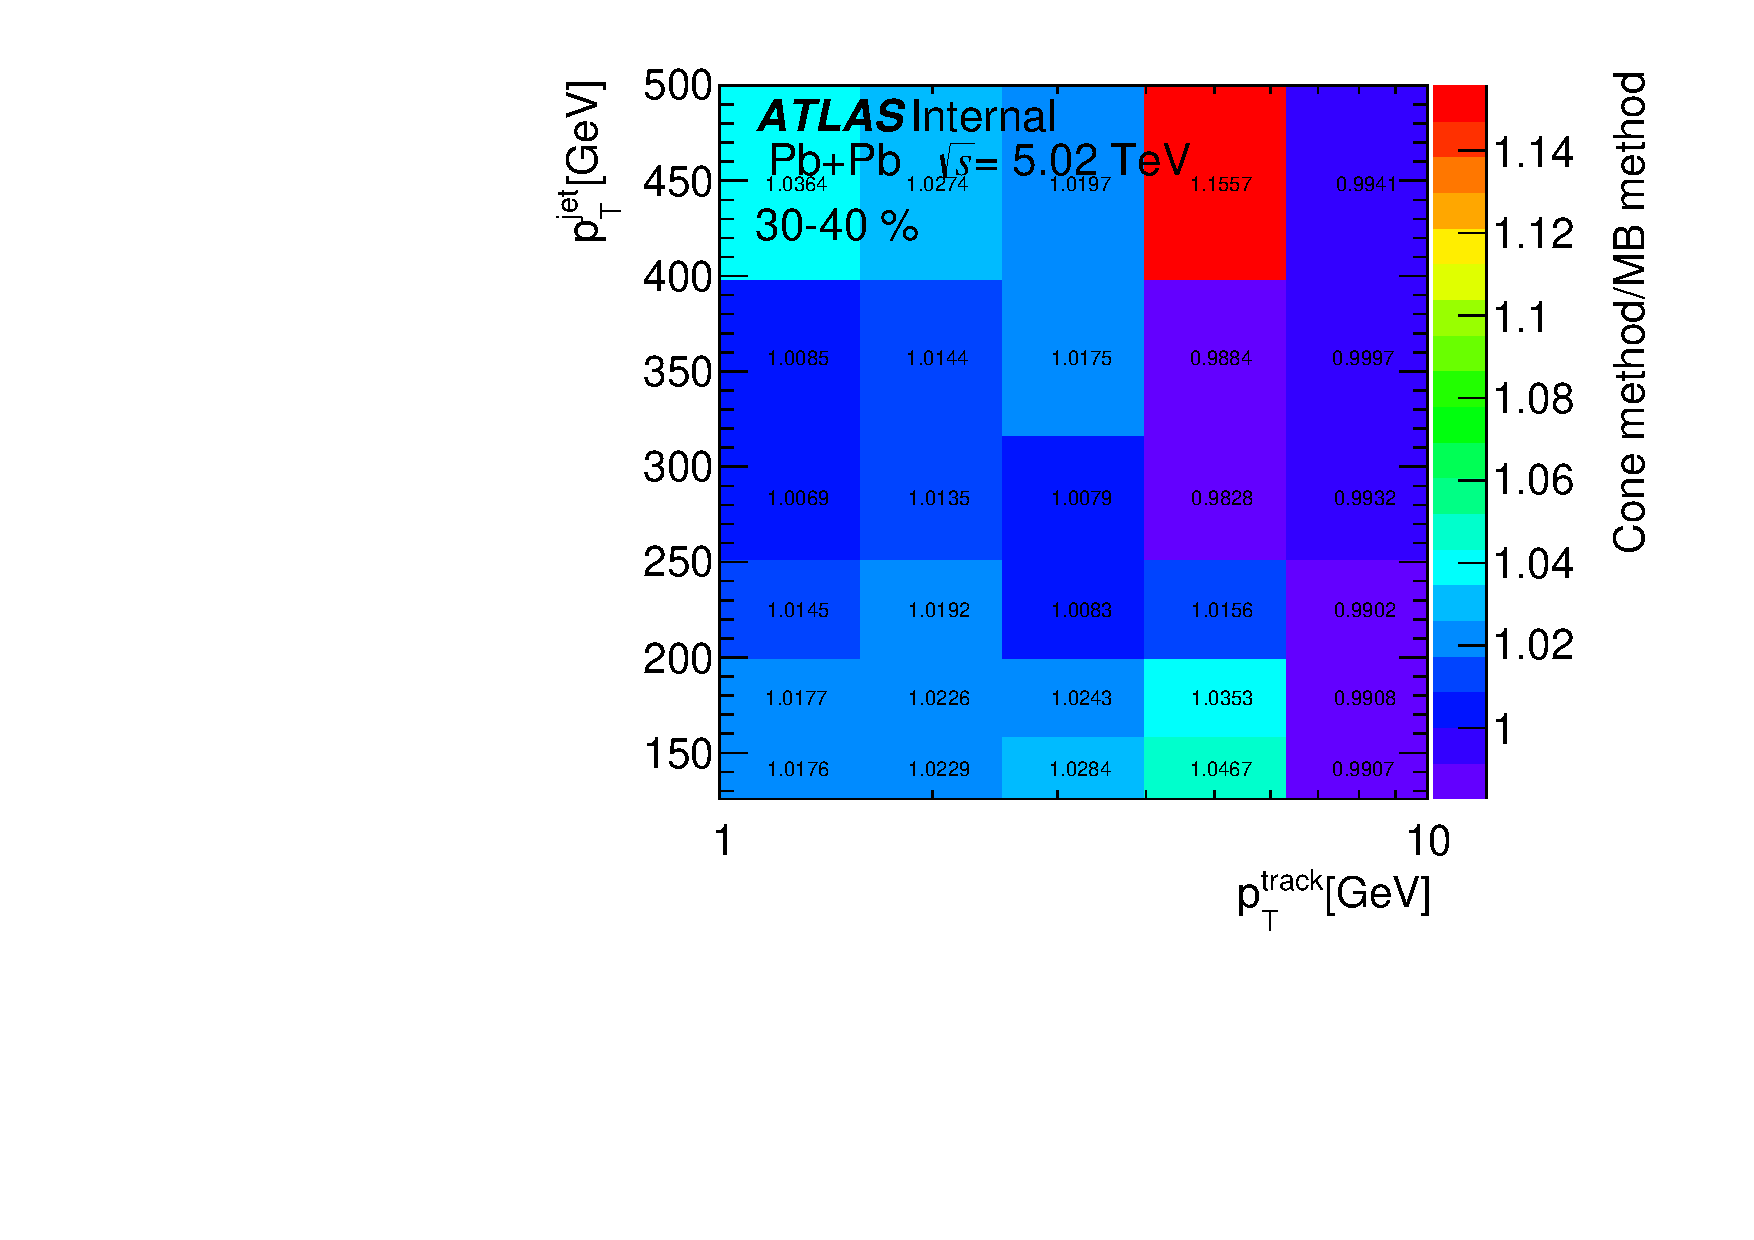
\includegraphics[width=0.55\textwidth]{figures_systematics/h_UE_comparison_cent3} \\
\end{tabular} }
   \caption{Comparison of the UE estimated by the two different methods in four collision centrality bins as a function of track and jet \pT.}
      \label{fig:UEuncert1}
\end{figure}

The estimated contribution from the UE needs to be corrected for the difference in the average UE yield at a given \pttrk\ between the $\eta$ position of the cone and $\eta$ position of the jet. This correction is based on the centrality-, \pttrk-, and $\eta$-dependent distribution of charged-particle yields in MB
data events. Separately, a correction is applied to the charged-particle UE estimate to account for the difference in the azimuthal particle density, due to elliptic flow, between the $\phi$ position of the cone and the $\phi$ position of the jet. This  utilizes a centrality- and \pttrk-dependent parameterization of the measured elliptic flow coefficients. The UE contribution is further corrected for the correlation between the actual UE yield underneath the jet and the jet energy resolution by the same method as used for default UE estimate.

\begin{figure}[h]
    \centerline{
       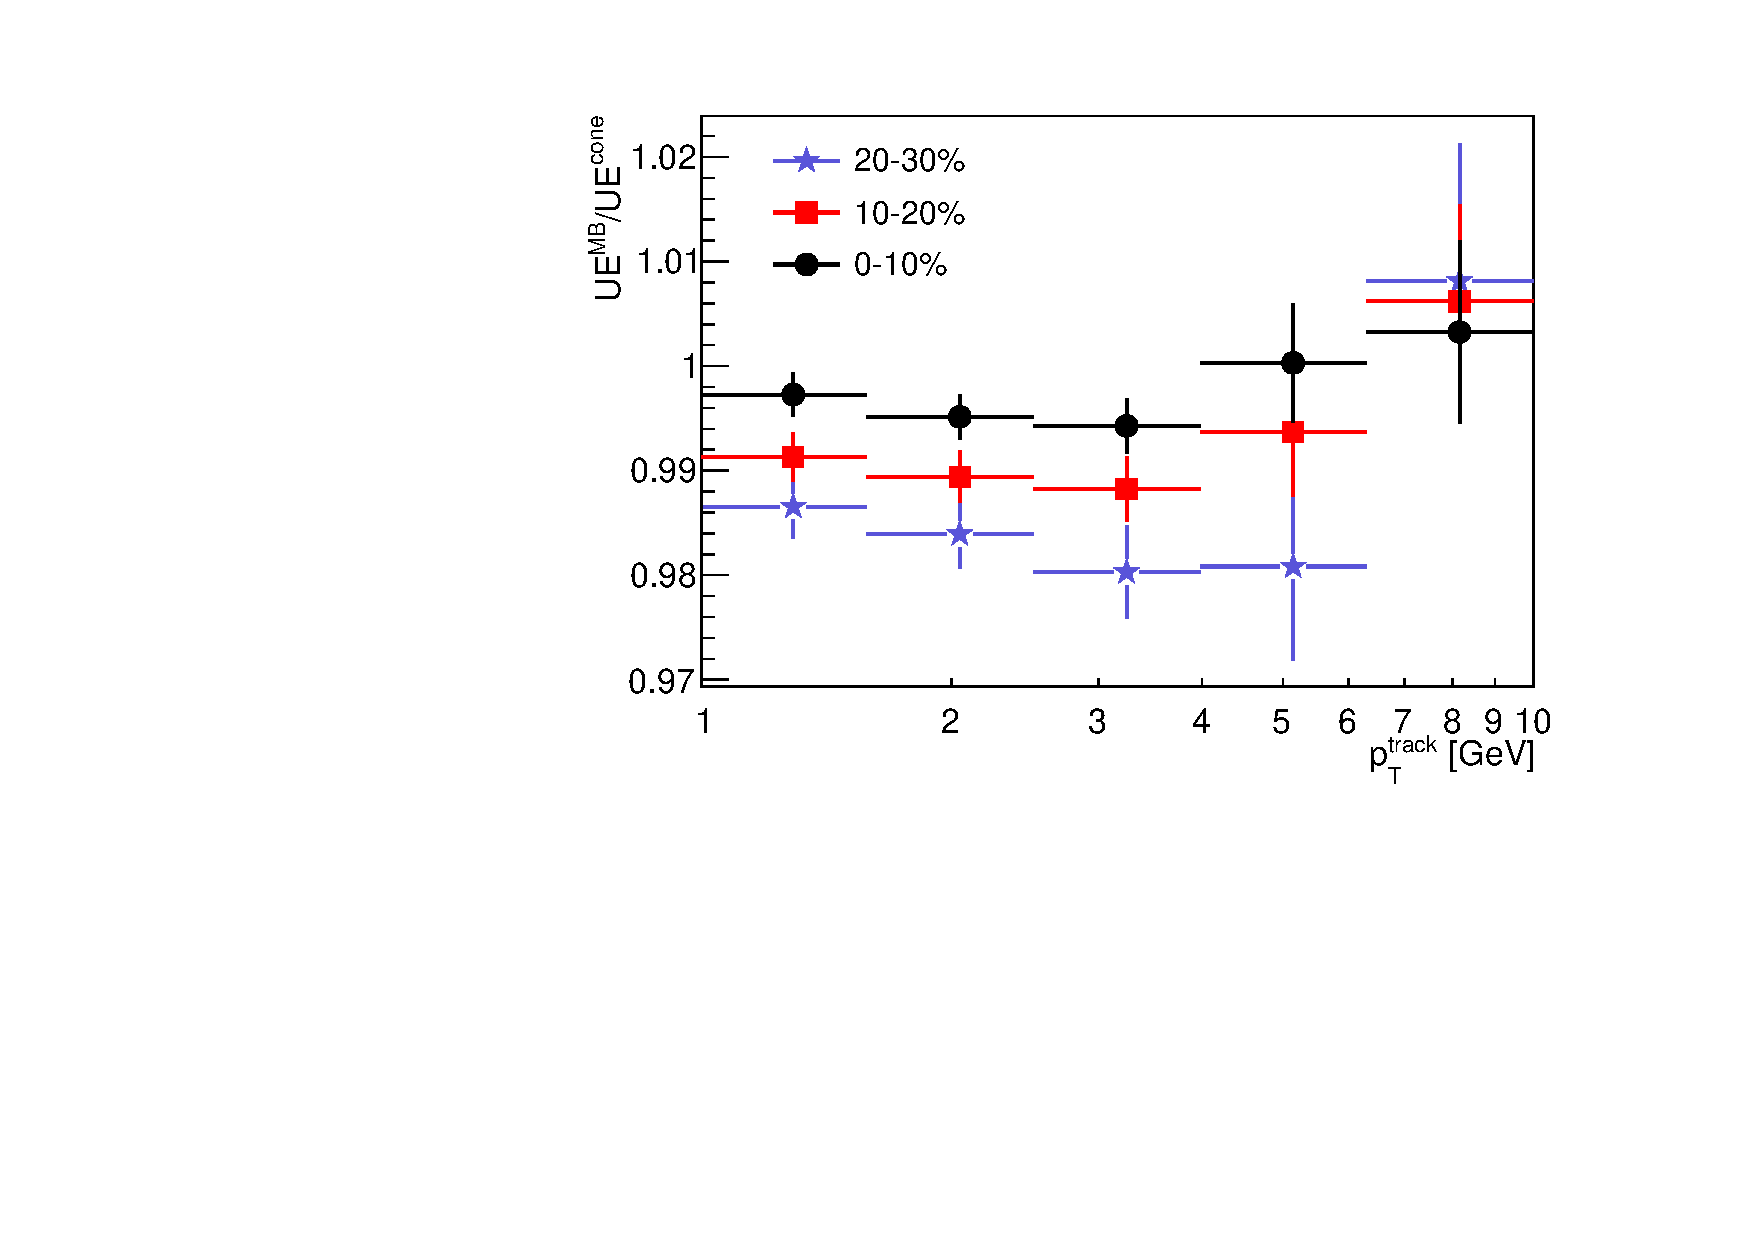
\includegraphics[width=0.75\textwidth]{figures_systematics/UE_uncert}
    }
    \caption{Comparison of the UE estimated by the two different methods in three collision centrality bins as a function of track \pT.}
    \label{fig:UEuncert2}
 \end{figure}

The difference between the two methods is shown in Fig.~\ref{fig:UEuncert1} and is found to be independent of jet \pT\ and exhibits a small centrality dependence. The uncertainty presented as the ratios between the two method averaged over jet \pT\ is shown in Fig.~\ref{fig:UEuncert2} is applied independent of \rvar\ and conservatively it is symmetrized. The absolute size of the uncertainty on the UE is typically small ($<<1$\%) however due to small signal-to-background ratio it is the dominant systematic uncertainty in central collisions, for lowest \pT\ tracks, and large \rvar.

%As it is discussed in Sec~\ref{sec:cuts_corrections} such UE estimates differ by construction in the rate of fake and secondary particles and also the UE from unmatched charged particles accounts for the effect of correlation between the JER and size of UE. For the purpose of evaluating systematic uncertainties, the impact of those two contributions is removed. This is done in the following two steps:
%\begin{enumerate}
%\item Based on the barcode that is available in MC samples the secondary particles, whose production is strongly correlated with jet, are removed.
%\item To suppress the effect when the UE underneath the jet is higher on average due to the convolution of steeply falling jet spectra and the JER, the UE from unmatched charged particles is estimated in intervals of corresponding truth jet \pT.    
%\end{enumerate}         

%\subsection{MC non-closure}
%To make sure that all the sources of systematic uncertainties were covered the systematic uncertainty from the ”non-closure” in the MC was also evaluated. It was 
%calculated as a deviation from unity of ratios of fully corrected and reconstructed fragmentation functions in MC %to the fragmentation functions
%evaluated at the truth level. 
%This uncertainty can be considered a measure of unknowns in the analysis, but it also includes fluctuations due to 
%the finite statistics in the MC which are used to evaluate it (especially in high \z\ \pttrk\ regions of
%the analysis.
%The systematic uncertainty is taken to be uncorrelated between \pbpb\ and \pp. This uncertainty is small as the
%closure is good (see Figure~\ref{fig:pbpbclosure}).  This systematic uncertainty is taken to be uncorrelated 
%between \pbpb\ and \pp.

\subsection{Correlations between the systematic uncertainties in \pbpb\ and \pp\ collisions}

Due to the common analysis and reconstruction procedure, and detector conditions, the systematic uncertainties are correlated between the \pp\ and
\pbpb\ collisions in most cases. Table~\ref{tab:systematics} summarizes correlations between \pp\ and \PbPb\ and also point-to-point correlations of individual distributions. The unfolding uncertainty is uncorrelated between the two systems because it
comes from the sensitivity of the unfolding to the starting MC distribution. In \pbpb\ collisions where the fragmentation is modified by the presence of the QGP, this sensitivity could be different than in \pp\ collisions where the fragmentation functions are quite similar to those in \pythiaeight~\cite{Aaboud:2017tke}. The impact of the modification of the fragmentation process in \PbPb\ compared to \pp\ and MC simulations is account for in the HI specific data-driven and centrality dependent uncertainty on the JES.

\begin{table}[h]
\begin{center}
\begin{tabular}{|c|c|c|c|}
\hline
uncertainty & \pp\ and \PbPb\ correlated & point-to-point correlated & one/two sided or symmetrized \\ \hline
JES (\pp) & yes & yes & two sided \\ \hline
JES (HI) & no & yes & two sided \\ \hline
JER & yes & yes & symmetrized \\ \hline
Track selection & yes & yes & one sided \\ \hline
Truth track definition & yes & yes & one sided \\ \hline
Material & yes & yes & one sided \\ \hline
Dense environment & yes & yes & one sided \\ \hline
Fake rate & yes & yes & symmetrized \\ \hline
Track momentum & yes & no & two sided \\ \hline
Unfolding & no & yes & one sided \\ \hline
UE subtraction & no & yes & symmetrized \\ \hline
% MC non-closure & no & no & symmetrized \\ \hline
\end{tabular}
\caption{Summary of correlation of different systematic uncertainties.}
\label{tab:systematics}
\end{center}
\end{table}

In the case where the systematic uncertainties are correlated, we evaluate \Rdptr\ ratios using the systematic variation from the nominal distributions in both \pp\ and \pbpb. The variation in the ratio is used as the systematic uncertainty. The variations in the ratios are summed in quadrature to get the total systematic uncertainty on the ratio.


